\documentclass[aspectratio=149]{beamer}

\usepackage{bm}
\usetheme{metropolis}           % Use metropolis theme
\title{Variational Inference in RKHS for Uncertainty Estimation in Deep Learning}
\date{\today}
\author{Luis Antonio Ortega Andrés\\
Simón Rodríguez Santana\\
Daniel Hernández Lobato\\}
\institute{Autonomous University of Madrid}
\usepackage[most]{tcolorbox}

\newtcolorbox{HighlightBoxFit}[1][]{%
   enhanced,
   hbox,
   %fontupper=\itshape,
   before    = \par\smallskip\centering,
   after     = \par,
   width     = 14cm,
   colback   = blue!5,
   colframe  = blue!40!white, 
   arc       = 4mm, 
   outer arc = 3.5mm, 
   #1}

\NeedsTeXFormat{LaTeX2e}
\usepackage{amsfonts}       % blackboard math symbols
\usepackage{amssymb,amsmath,amsthm}
\usepackage{braket}
\usepackage{booktabs} % for professional tables
\usepackage{tabularx}

\usefonttheme{professionalfonts} % required for mathspec
\usepackage{mathspec}
\setsansfont[BoldFont={Fira Sans}]{Fira Sans Light}

\newcommand{\h}[1]{\color{orange}\textbf{#1}}

\DeclareMathOperator*{\argmax}{arg\,max}
\DeclareMathOperator*{\argmin}{arg\,min}

\colorlet{shadecolor}{gray!40}
\begin{document}
  \maketitle


    {\setbeamercolor{background canvas}{bg=white}
      \begin{frame}{}
        \begin{figure}
            \centering
            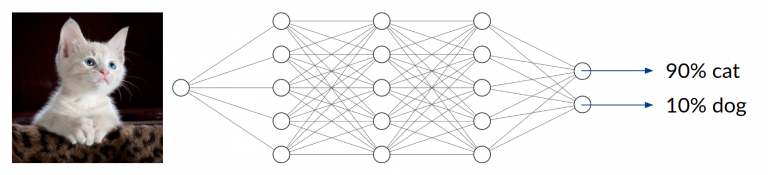
\includegraphics[width = 0.8\textwidth]{slides_imgs/Bildschirmfoto-vom-2019-10-01-11-03-08-768x175.png}
            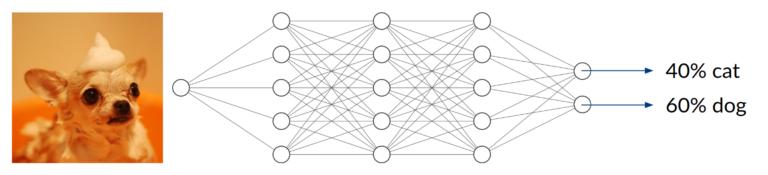
\includegraphics[width = 0.8\textwidth]{slides_imgs/uncertainty-quantification-dog-768x175.png}
        \end{figure}
    \end{frame}}
    
    {\setbeamercolor{background canvas}{bg=white}
      \begin{frame}{}
        \begin{figure}
            \centering
            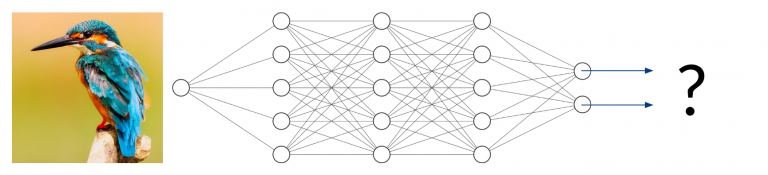
\includegraphics[width = 0.8\textwidth]{slides_imgs/Bildschirmfoto-vom-2019-10-01-11-03-18-768x175.png}
        \end{figure}
        \pause
        \begin{center}
        \textbf{Deep learning methods are unable to quantify the uncertainty of their predictions!}
        \end{center}
    \end{frame}}
    
    {\setbeamercolor{background canvas}{bg=white}
      \begin{frame}{}
      \textbf{Straight-forward solution}: Using a Bayesian model.
        \begin{figure}
            \centering
            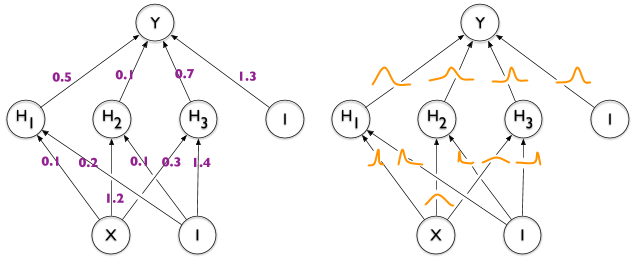
\includegraphics[width = 0.8\textwidth]{slides_imgs/Bayesian-Neural-Network.png}
        \end{figure}
    \end{frame}}

    \begin{frame}
        Making predictions \textbf{requires the posterior} over the parameters of the model \(\bm{\theta}\):
        \[
            p(y^\star | \mathbf{x}^\star, \mathcal{D}) = \int p(y^\star | \mathbf{x}^\star, \bm{\theta}) p(\bm{\theta} | \mathcal{D}) \ d\bm{\theta}\,,
        \]
        where \( p(\bm{\theta} | \mathcal{D}) \) is \textbf{intractable for complex models}.
    \end{frame}


    \begin{frame}
        \begin{center}
            Approximate  \( p(\bm{\theta} | \mathcal{D}) \) by something simpler \(q(\bm{\theta})\).
            \onslide<2>
            {
                \[
                    \Bigg\Downarrow
                \]
                \textbf{Poor performance in many cases.}
            }
        \end{center}
    \end{frame}

    \begin{frame}{Approach}

        \begin{enumerate}[<+->]
            \item Learn a DL \textbf{deterministic} model \(h\).
            \begin{center}
                \h{High Performance - No Uncertainty}
            \end{center}
            \item  Variational Sparse Gaussian Processes with \textbf{posterior mean \(h\)}.
            \begin{center}
                \h{High Performance - Uncertainty Estimation}
            \end{center}
            \item Optimize parameters using function-space VI.
        \end{enumerate}

    \end{frame}
        \begin{frame}{Gaussian Processes}
        \begin{center}\color{orange}
            \textbf{Uncertainty Estimation in function-space}
        \end{center}
        {\color{shadecolor}
        Given a mean \(m(\cdot)\) and covariance function \(\kappa(\cdot, \cdot)\), defines a \textbf{Gaussian prior over function evaluations}:
        \[
        p(f(\mathbf{x})) = \mathcal{N}(m(\mathbf{x}), K(\mathbf{x}, \mathbf{x}))\,.
        \]
        \[
        f \sim \mathcal{G}\mathcal{P}(m, K)\,.
        \]
        }
    \end{frame}
    \begin{frame}{Gaussian Processes}
        \begin{center}\color{shadecolor}\textbf{Uncertainty Estimation in function-space}
        \end{center}
        {\color{black}
        Given a mean \(m(\cdot)\) and covariance function \(\kappa(\cdot, \cdot)\), defines a {\color{orange}\textbf{Gaussian prior over function evaluations}}:
        \[
        p(f(\mathbf{x})) = \mathcal{N}(m(\mathbf{x}), \kappa(\mathbf{x}, \mathbf{x}))\,.
        \]
        \[
        f \sim \mathcal{G}\mathcal{P}(m, \kappa)\,.
        \]
        }
    \end{frame}
    \begin{frame}{Gaussian Processes}
    Set of observations \((\mathbf{X}, \mathbf{y})\), the \textbf{predictive distribution} is Gaussian
        \[
        p(y^\star | \mathbf{x}^\star, \mathbf{X}, \mathbf{y}) = \mathcal{N}(m^\star(\mathbf{x}^\star), K(\mathbf{x}^\star, \mathbf{x}^\star))\,.
        \]
        \pause
        \[
        m^\star(\mathbf{x}^\star) = \kappa(\mathbf{x}^\star, \mathbf{X})(\kappa(\mathbf{X}, \mathbf{X}) + \sigma^2 \bm{I})^{-1}(\mathbf{y} - m(\mathbf{x}^\star))\,,
        \]
        \[
        K(\mathbf{x}^\star, \mathbf{x}^\star) = \kappa(\mathbf{x}^\star, \mathbf{x}^\star) - \kappa(\mathbf{x}^\star, \mathbf{X})(\kappa(\mathbf{X}, \mathbf{X}) + \sigma^2 \bm{I})^{-1}\kappa(\mathbf{X},  \mathbf{x}^\star)\,.
        \]
        \begin{center}
            \emph{Gaussian noise with variance \(\sigma^2\) is considered for the targets}
        \end{center}
    \end{frame}

    \begin{frame}{Sparse Variational Gaussian Processes}
    \begin{center}
    Define a set of \emph{inducing locations} \(\mathbf{Z} \subset \mathbb{R}^D\) that ``summarize'' the training inputs \(\mathbf{X}\). 
    \end{center}

    \begin{center}
        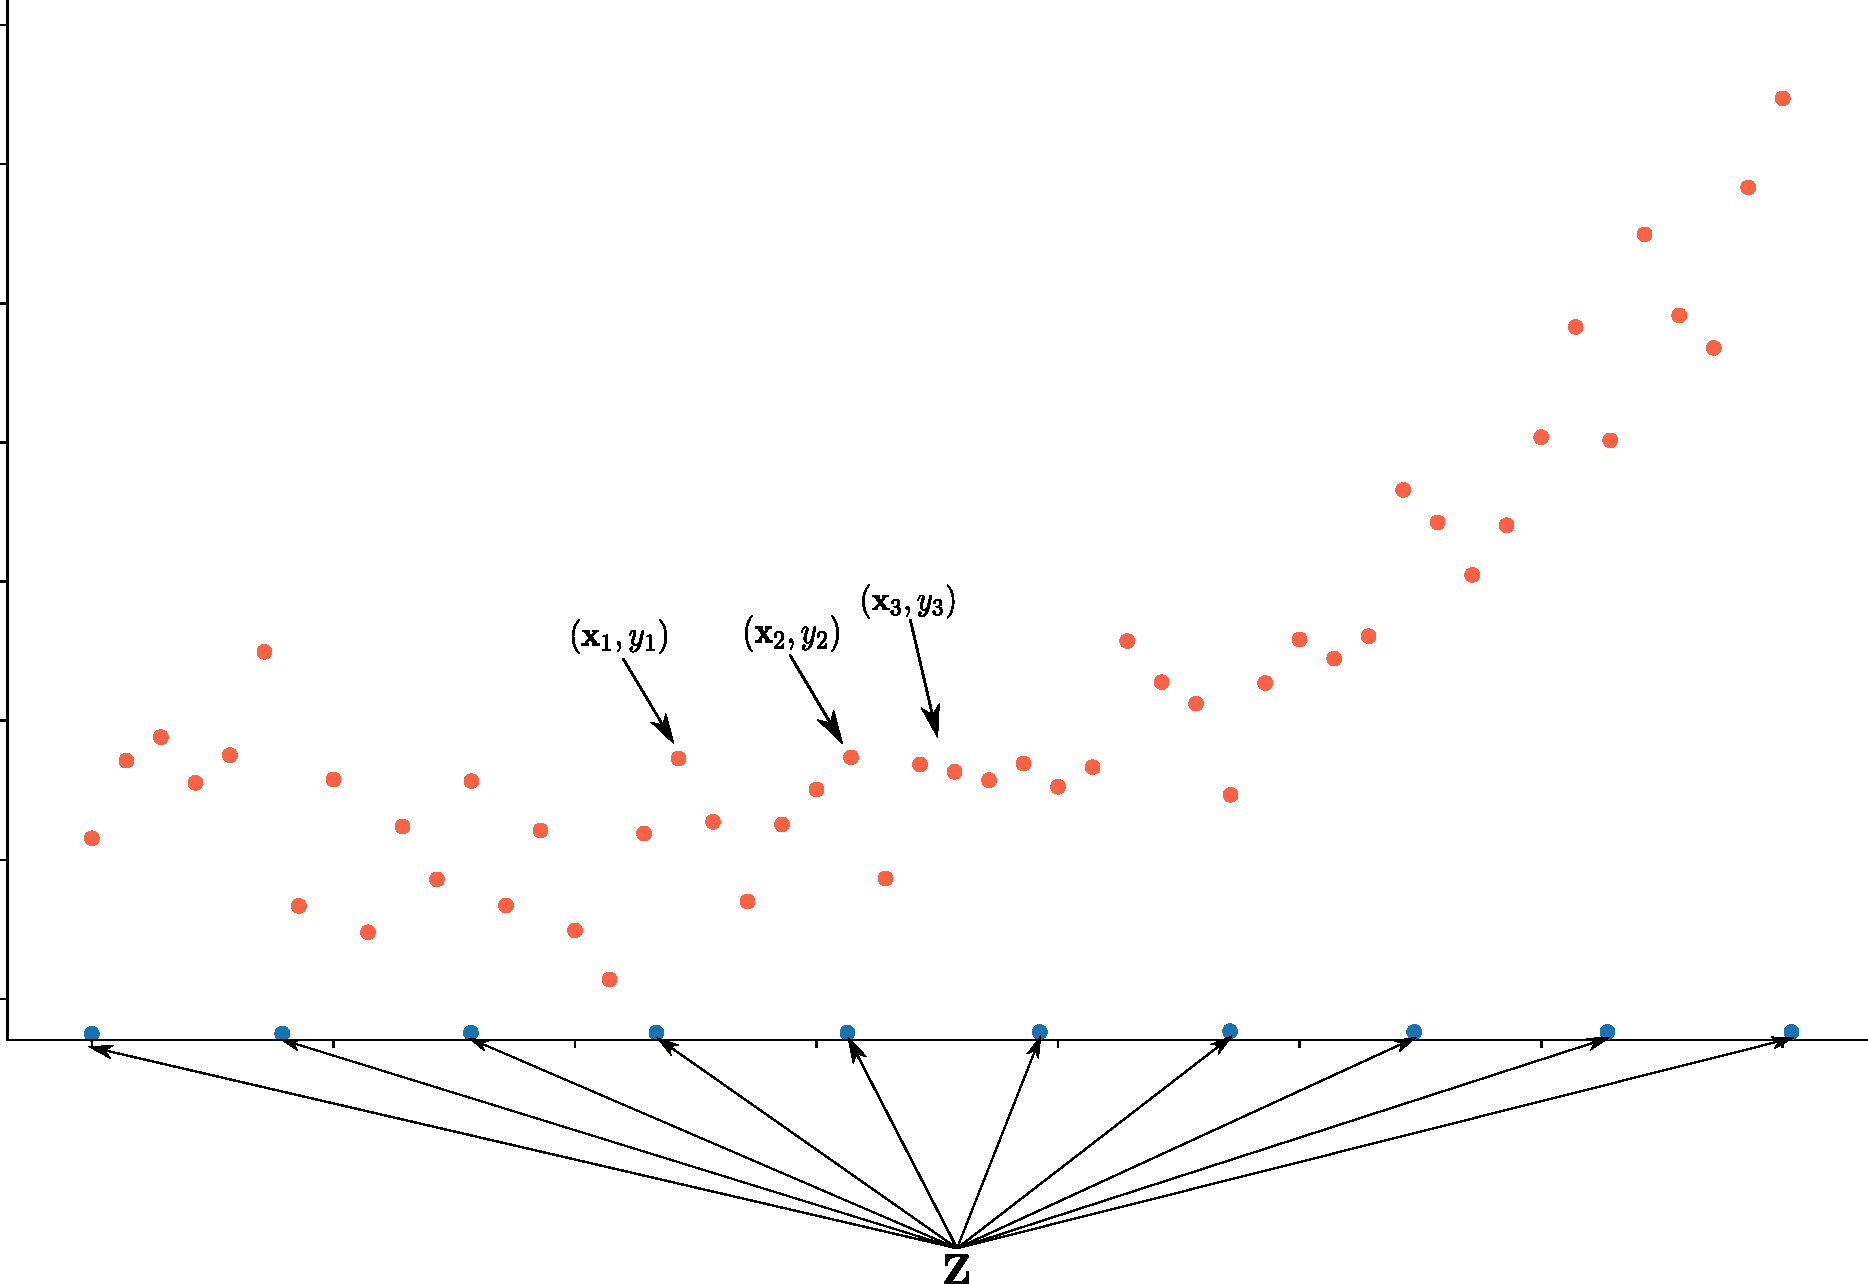
\includegraphics[width=0.7\textwidth]{slides_imgs/GP_inducing_1.pdf}
    \end{center}
    \end{frame}
    \begin{frame}{Sparse Variational Gaussian Processes}
    \begin{center}
    With \(\mathbf{u} = f(\mathbf{Z})\), the posterior \(p(\mathbf{u}|\mathbf{X}, \mathbf{y})\) is approximated with variational distribution \(q(\mathbf{u}) = \mathcal{N}(\bm{\mu}, \bm{\Sigma})\).
    \end{center}

    \begin{center}
        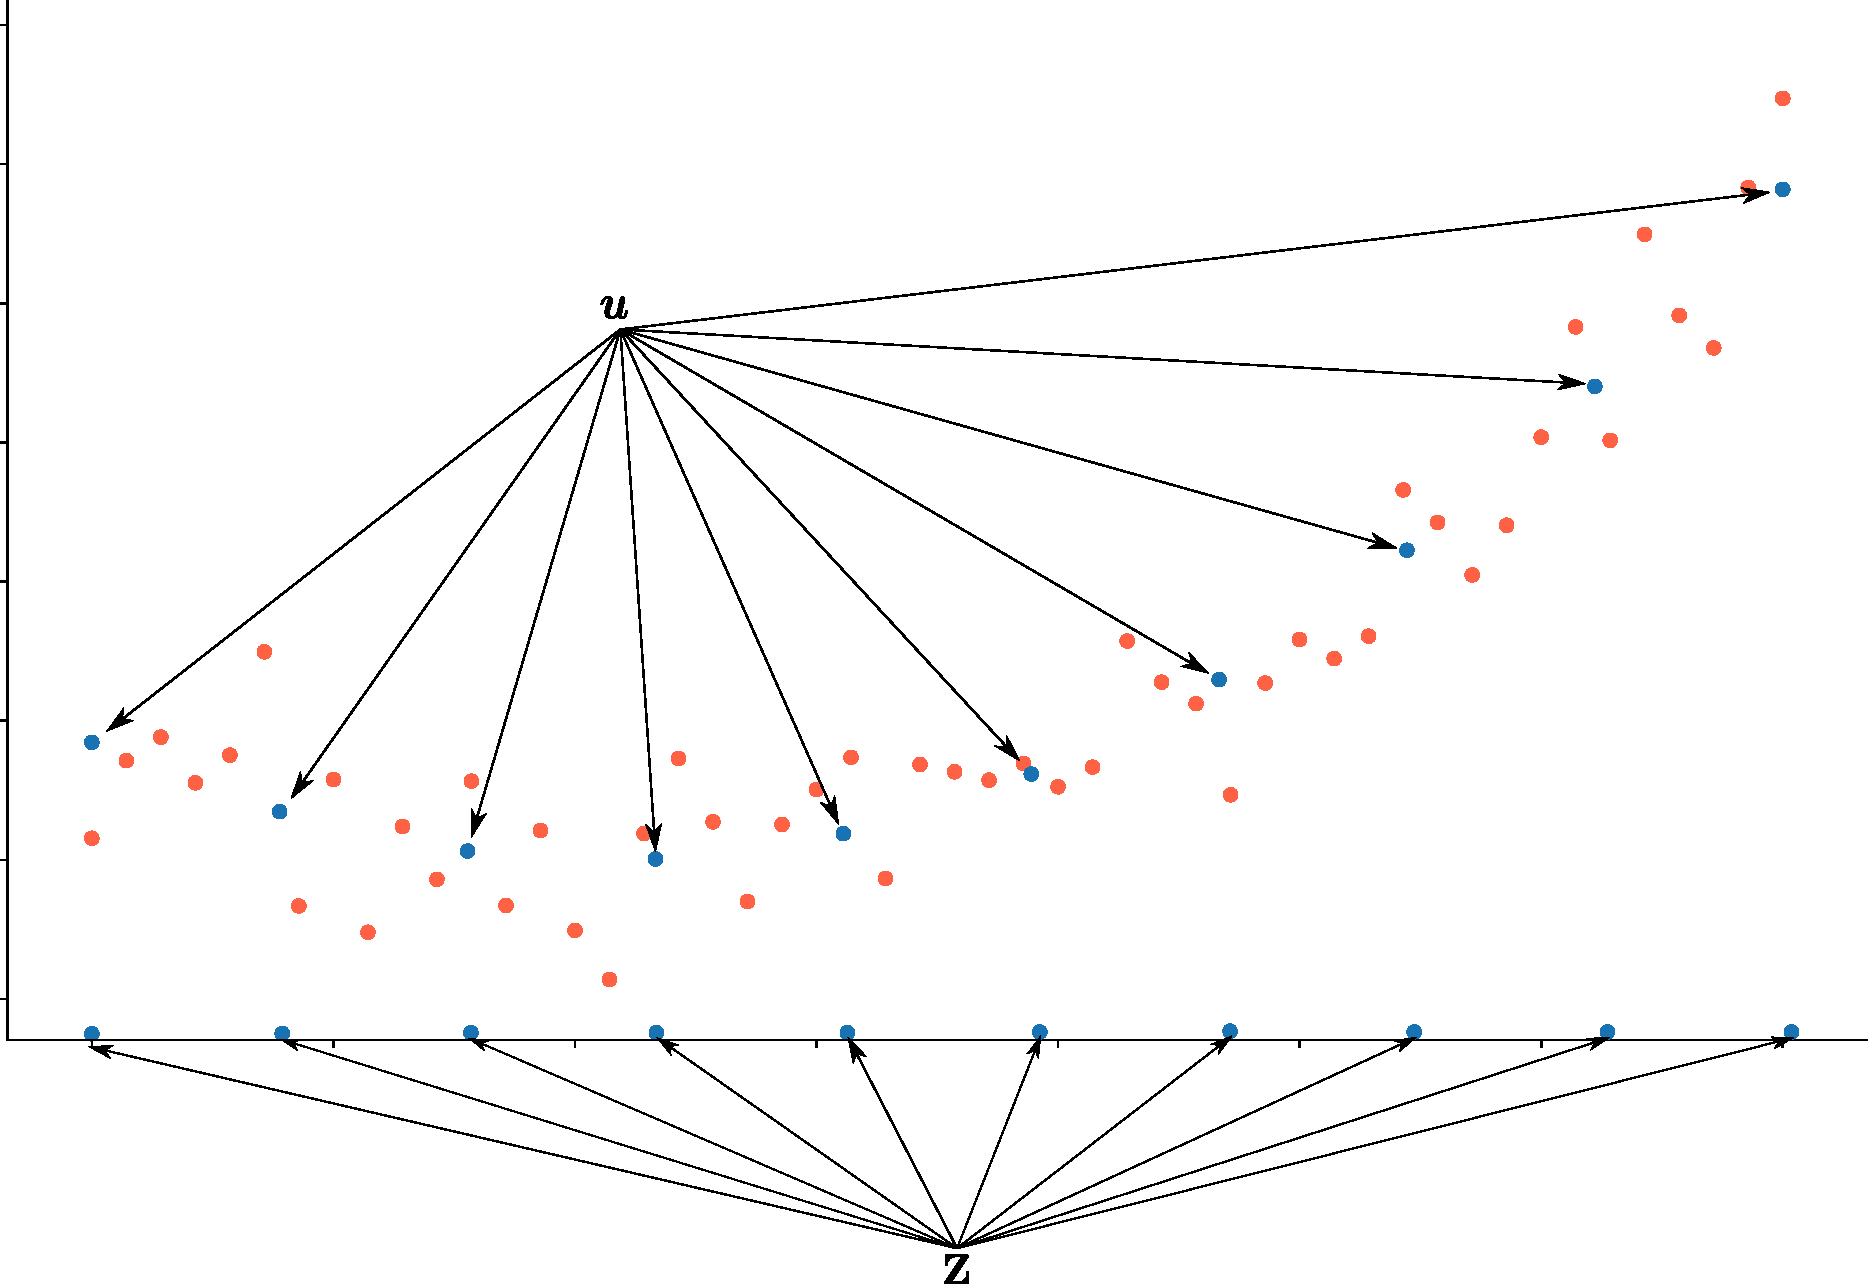
\includegraphics[width=0.7\textwidth]{slides_imgs/GP_inducing_2.pdf}
    \end{center}
    \end{frame}

    \begin{frame}{Sparse Variational Gaussian Processes}
    \begin{center}
    The inducing points can be marginalized in closed form to make predictions.
    \end{center}
    
    \begin{center}
        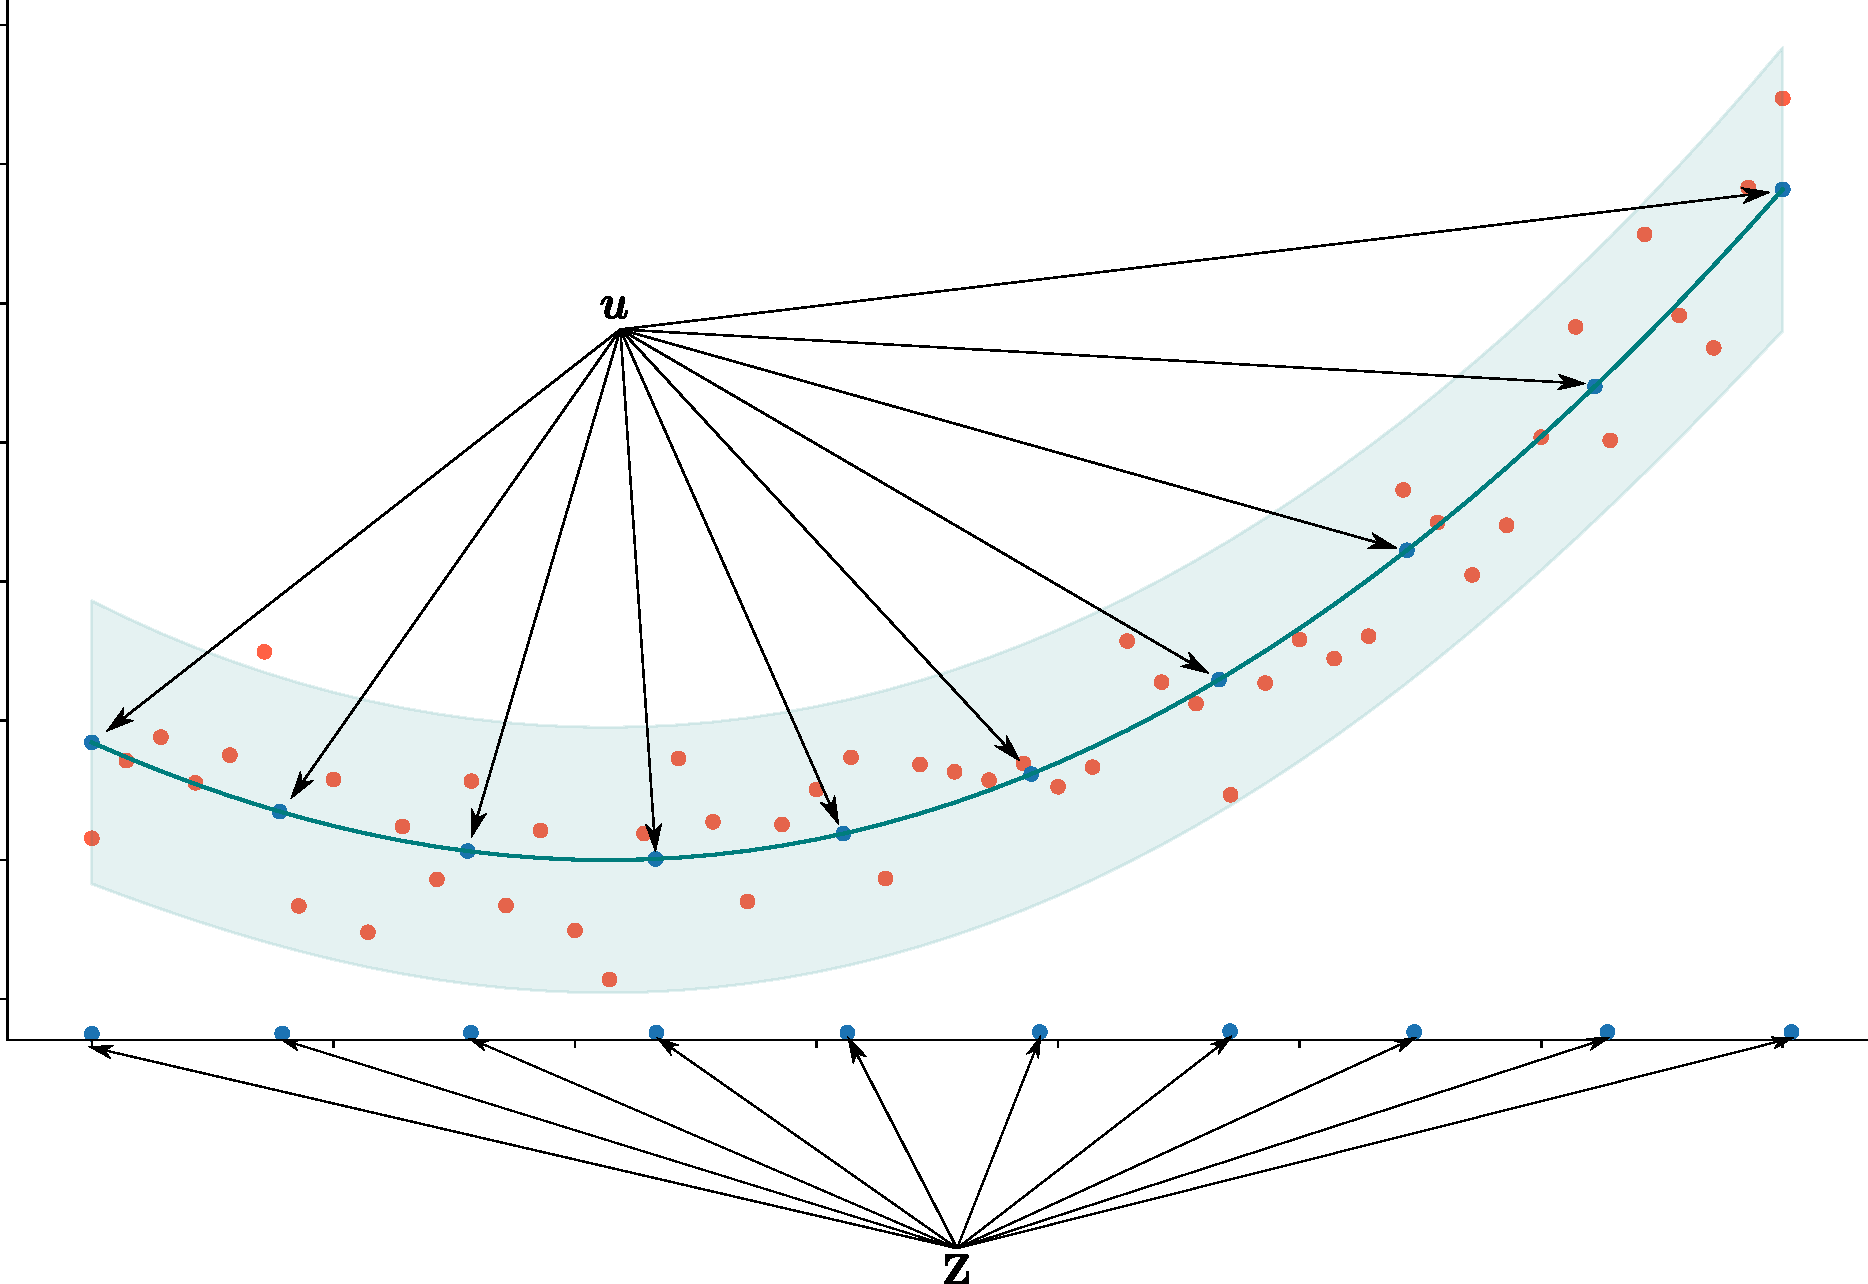
\includegraphics[width=0.7\textwidth]{slides_imgs/GP_inducing_3.pdf}
    \end{center}
    \end{frame}

    % \[
    % m^\star(\mathbf{x}^\star) = \kappa(\mathbf{x}^\star, \mathbf{Z})\kappa(\mathbf{Z}, \mathbf{Z})^{-1}\bm{\mu}
    % \]
    % \[
    % \begin{aligned}
    % K(\mathbf{x}^\star, \mathbf{x}^\star) &= \kappa(\mathbf{x}^\star, \mathbf{x}^\star) - \kappa(\mathbf{x}^\star, \mathbf{Z})\kappa(\mathbf{Z}, \mathbf{Z})^{-1}\kappa(\mathbf{Z},  \mathbf{x}^\star)\\
    % &+ \kappa(\mathbf{x}^\star, \mathbf{Z})\kappa(\mathbf{Z}, \mathbf{Z})^{-1}\bm{\Sigma}\kappa(\mathbf{Z}, \mathbf{Z})^{-1}\kappa(\mathbf{Z},  \mathbf{x}^\star)
    % \end{aligned}
    % \]

    % \begin{frame}
    %     The exact posterior can be computed with access to the whole dataset \(\mathbf{X}\) as:
    %     \[
    %     P(\bm{u}|\mathbf{X}, \mathbf{y}) = \mathcal{N}(\bm{\mu}^\star, \bm{\Sigma}^\star)
    %     \]
    %     \[
    %     \bm{\mu}^\star = \sigma^{-2}K(\mathbf{Z}, \mathbf{Z})\Sigma K(\mathbf{Z}, \mathbf{X})
    %     \]
    %     \[
    %     \bm{\Sigma}^\star = K(\mathbf{Z}, \mathbf{Z})\Sigma K(\mathbf{Z}, \mathbf{Z})
    %     \]
    %     \[
    %     \Sigma = (K(\mathbf{Z}, \mathbf{Z}) - \sigma^{-2}K(\mathbf{Z}, \mathbf{X})K(\mathbf{X}, \mathbf{Z}))^{-1}
    %     \]
    % \end{frame}

    \begin{frame}{Dual representation of Gaussian Processes}

        A \textbf{RKHS} \(\mathcal{H}\) is a Hilbert space of functions satisfying the \textbf{reproducing property}: \(\forall \mathbf{x} \in \mathcal{X} \ \exists \phi_{\mathbf{x}} \in \mathcal{H}\) such that \(\forall g \in \mathcal{H}, g(\mathbf{x}) = \braket{\phi_{\mathbf{x}}, g} \).
        
        \pause
        
        A \textbf{Gaussian process} \(f\sim \mathcal{GP}(m, K)\) has a \textbf{dual representation} in a RKHS as: there exists \(\mu \in \mathcal{H}\) and a linear semi-definite positive operator \(\Sigma:\mathcal{H} \to \mathcal{H}\) such that, for any \(\mathbf{x}, \mathbf{x}' \in \mathcal{X}\), \(\exists \phi_{\mathbf{x}}, \phi_{\mathbf{x}'}\), verifying
        \[
            m(\mathbf{x}) = \braket{\phi_{\mathbf{x}}, \mu}, \quad K(\mathbf{x}, \mathbf{x}') = \braket{\phi_{\mathbf{x}}, \Sigma(\phi_{\mathbf{x}'})}\,.
        \]
        
        \pause 
        
        We write \(f \sim \mathcal{N}(\mu, \Sigma)\), which is a \textbf{Gaussian measure} in the RKHS.
    \end{frame}

    \begin{frame}
        This characterization in the RKHS allows the \textbf{rethink Gaussian Processes as Gaussian Measures} in the Hilbert space:
        \[
        p(f) = \mathcal{N}(\mu, \Sigma)
        \]
        \pause
        The \textbf{posterior measure} can be specified as a \textbf{Gaussian}:
        \[
        p(f|\mathbf{y}) = \mathcal{N}(\mu^\star, \Sigma^\star)
        \]
        \vspace{0.2cm}
        \[
        \mu^\star = \kappa(\cdot, \mathbf{X})(\kappa(\mathbf{X}, \mathbf{X}) + \sigma^2 \bm{I})^{-1}(\mathbf{y} - m(\cdot))
        \]
        \[
        \Sigma^\star = I - \phi_{\mathbf{X}}^T(\kappa(\mathbf{X}, \mathbf{X}) + \sigma^2 \bm{I})^{-1}\phi_{\mathbf{X}}
        \]
    \end{frame}

    \begin{frame}
        \textbf{Theorem}. A SVGP is equivalent to restricting the mean and covariance functions in the RKHS to
        \[
            \tilde{\mu} = \Phi_{\mathbf{Z}}(\bm{a}) \quad \text{and} \quad \tilde{\Sigma} = I + \Phi_{\mathbf{Z}}\bm{A}\Phi_{\mathbf{Z}}^T\,,
        \]
        where \(\Phi_{\mathbf{Z}}: \mathbb{R}^M \to \mathcal{H} \) is defined as 
        \[\Phi_{\mathbf{Z}}(\bm{a}) = \sum_{m=1}^{M} a_m \phi_{\mathbf{z}_m}\,, \quad\text{ and }\quad \Phi_{\mathbf{Z}}\bm{A}\Phi_{\mathbf{Z}}^T= \sum_{i=1}^{M}\sum_{j=1}^M\phi_{\mathbf{z}_i} A_{i,j} \phi_{\mathbf{z}_j}^T
        \]
        where \(\bm{A} \in \mathbb{R}^{M\times M}\) such that \(\tilde{\Sigma} \geq 0\).

    {\let\thefootnote\relax\footnote{{Cheng, C.A. and Boots, B., 2016. Incremental variational sparse Gaussian process regression. Advances in Neural Information Processing Systems, 29.}}}
    \end{frame}

    \begin{frame}
        A SVGP can be \textbf{\color{orange}generalized} with mean and covariance functions of the dual representation in the RKHS to
        \[
            \tilde{\mu} = \Phi_{\color{red}\mathbf{Z}_\alpha}(\bm{a}) \quad \text{and} \quad \tilde{\Sigma} = I + \Phi_{\color{blue}\mathbf{Z}_\beta }\bm{A}\Phi_{\color{blue}\mathbf{Z}_\beta}^T\,,
        \]
        where \(\color{red}\mathbf{Z}_\alpha\) and \(\color{blue}\mathbf{Z}_\beta\) are two sets of inducing locations.
        
    {\let\thefootnote\relax\footnote{{Cheng, C.A. and Boots, B., 2017. Variational inference for Gaussian process models with linear complexity. Advances in Neural Information Processing Systems, 30.}}}
    \end{frame}

     {\setbeamercolor{background canvas}{bg=white}\begin{frame}
        \begin{center}
            \textbf{Comparison between models with shared and decoupled basis}
        \end{center}
        \begin{figure}
            \centering
            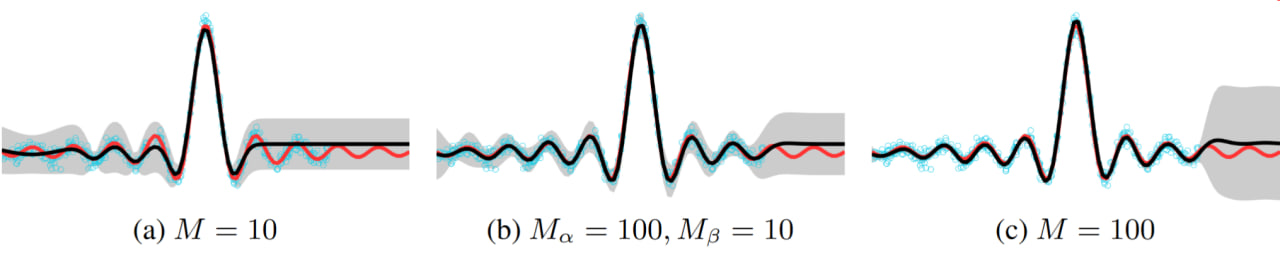
\includegraphics[width = 0.96\textwidth]{slides_imgs/decoupled.jpg}
        \end{figure}
        
        \begin{itemize}
            \item (a) and (c) denote the models with shared basis of size \(M\).
            \item (b) denotes the model of decoupled basis with size (\(M_\alpha, M_\beta\)).
        \end{itemize} 

        {\let\thefootnote\relax\footnote{{Figure from Cheng, C.A. and Boots, B., 2017. Variational inference for Gaussian process models with linear complexity. Advances in Neural Information Processing Systems, 30.}}}
    \end{frame}}


    \begin{frame}{Variational Optimization}

        SVGPs are optimized using the Evidence Lower Bound:
        \[
        \text{KL}\big(p(\mathbf{f}, \mathbf{u}| \mathbf{y})|q(\mathbf{f}, \mathbf{u})\big) = \log p(\mathbf{y})\underbrace{-\  \mathbb{E}_{q(\mathbf{f})}[ \log p(\mathbf{y} | \mathbf{f})] + \text{KL}\big(q(\mathbf{u})|p(\mathbf{u})\big)}_{-ELBO}
        \]
        with \(\mathbf{f} =f(\mathbf{X})\) and \(\mathbf{u} = f(\mathbf{Z})\).
        
        \pause
        Which is \textbf{equivalent} to optimize the ELBO in function-space
        \[
        \text{KL}\big(p(f| \mathbf{y})|q(f)\big) = \log p(\mathbf{y})\underbrace{ - \ \mathbb{E}_{q(f)}[ \log p(\mathbf{y} | f)] + \text{KL}\big(q(f)|p(f)\big)}_{-ELBO}
        \]   
        {\let\thefootnote\relax\footnote{{Cheng, C.A. and Boots, B., 2016. Incremental variational sparse Gaussian process regression. Advances in Neural Information Processing Systems, 29.}}}
    \end{frame}

    \begin{frame}{Variational Optimization}
        Optimizing the ELBO in the Hilbert space:
        \[
        \max_{q(f)}\  \mathcal{L} (q(f)) = \max_{q(f)}\ \mathbb{E}_{q(f)} \left[ \log p(\mathbf{y}|f)\right] - \text{KL}\left(q|p\right)\,.
        \]
        Where
        \[
            \text{KL}\left(q | p\right) = \underbrace{\frac{1}{2} \bm{a}^T \bm{K}_{\alpha} \bm{a}}_{\bm{a}, \mathbf{Z}_\alpha} +  \underbrace{\frac{1}{2} \log |\bm{I} - \bm{K}_{\beta} (\bm{A} + \bm{K}_{\beta})^{-1}| + \frac{1}{2} \text{tr}\left( \bm{K}_\beta\bm{A}^{-1} \right)}_{\bm{A}, \mathbf{Z}_\beta}
        \]
        and \(\mathbb{E}_{q(f)}\left[ \log p(\mathbf{y}|f)\right] \) can be computed in regression and estimated in classification.
    \end{frame}

    \begin{frame}{Fixing the Mean Function}
        If the kernel \(\kappa(\cdot, \cdot)\) is {\color{orange}\textbf{universal}}, then, \(\forall \epsilon > 0\), there exists a set of \(M_\alpha\) points \(\mathbf{Z}_\alpha \subset \mathbb{R}^D\) and coefficients \(\bm{a}\in \mathbb{R}^{M_\alpha}\), such that
        \[
            d_{\mathcal{H}}(h, \Phi_{\mathbf{Z}_\alpha}(\bm{a})) \leq \epsilon, \quad\text{ with }\quad \Phi_{\mathbf{Z}_\alpha}(\bm{a}) := \sum_{m=1}^{M_\alpha} a_m \phi_{\mathbf{z}_m}\,.
        \]
    \end{frame}

    \begin{frame}
        For any \(\epsilon > 0\), there exists a set of \(M_\alpha\) inducing points \(\mathbf{Z}_{\alpha} \subset \mathbb{R}^D\) and \(\bm{a} \in \mathbb{R}^{M_\alpha}\)\pause\ such that the corresponding decoupled sparse Gaussian process corresponds to \(\mathcal{GP}(m^\star, K^\star)\):
        \[
            \begin{aligned}
                m^{\star}(\mathbf{x}) &= \kappa(\mathbf{x}, \mathbf{Z}_\alpha)\bm{a}\,, \\
                K^{\star}(\mathbf{x}, \mathbf{x}') &= \kappa(\mathbf{x}, \mathbf{x}') +  \kappa(\mathbf{x}, \mathbf{Z}_\beta)\bm{A}^{-1} \kappa(\mathbf{Z}_\beta, \mathbf{x}')\,,
            \end{aligned}
        \]
        \pause
        where \(\mathbf{Z}_{\beta} \subset \mathbb{R}^D\) is a set of \(M_\beta\) inducing points, \(\bm{A} \in \mathbb{R}^{M_\beta \times M_\beta}\) such that \(\tilde{\Sigma} \geq 0\) and it verifies 
        \[
        d_{\mathcal{H}}(h, m^\star) \leq \epsilon\,
        \]
    \end{frame}
    \begin{frame}
        \begin{center}
            \textbf{Distributions over function-space with fixed mean to \(h\).}
        \end{center}
        \pause
        \begin{center}
        \textbf{Parameters}: \(\mathbf{Z}_{\beta} \subset \mathbb{R}^D\) and \(\bm{A} \in \mathbb{R}^{M_\beta \times M_\beta}\) (such that \(\tilde{\Sigma} \geq 0\)).
        \end{center}
        \pause
        \begin{center}  
        Gaussian process posterior approximation \(\mathcal{GP}(m^\star, K^\star)\):
        \end{center}
        \[
            \begin{aligned}
                m^{\star}(\mathbf{x}) &\approx h(\mathbf{x})\,, \\
                K^{\star}(\mathbf{x}, \mathbf{x}') &=\kappa(\mathbf{x}, \mathbf{x}') +  \kappa(\mathbf{x}, \mathbf{Z}_\beta)\bm{A}^{-1} \kappa(\mathbf{Z}_\beta, \mathbf{x}')\,,
            \end{aligned}
        \]
    \end{frame}

    \begin{frame}{Diagram - Distribution over function-space}
        \begin{figure}[h]
        	\begin{center}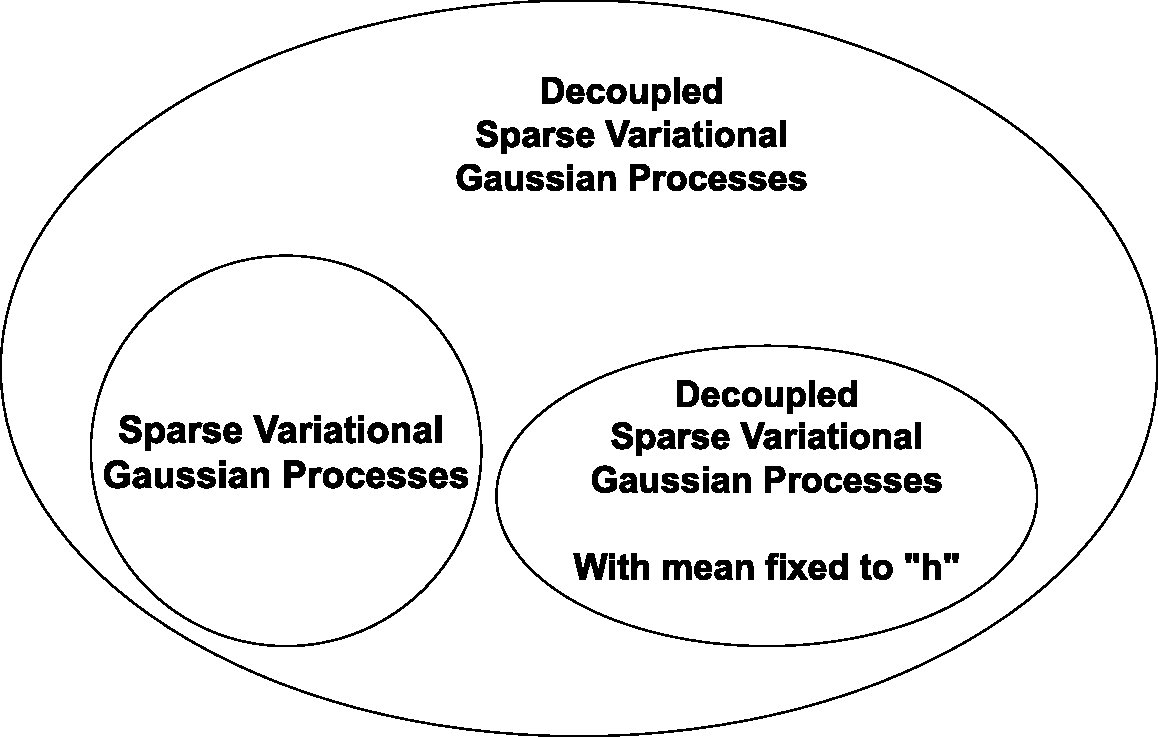
\includegraphics[width=0.90\textwidth]{slides_imgs/diagram.pdf} 
        	\end{center}
        \end{figure}
    \end{frame}
    \begin{frame}{Diagram - Distribution over function-space}
        \begin{figure}[h]
        	\begin{center}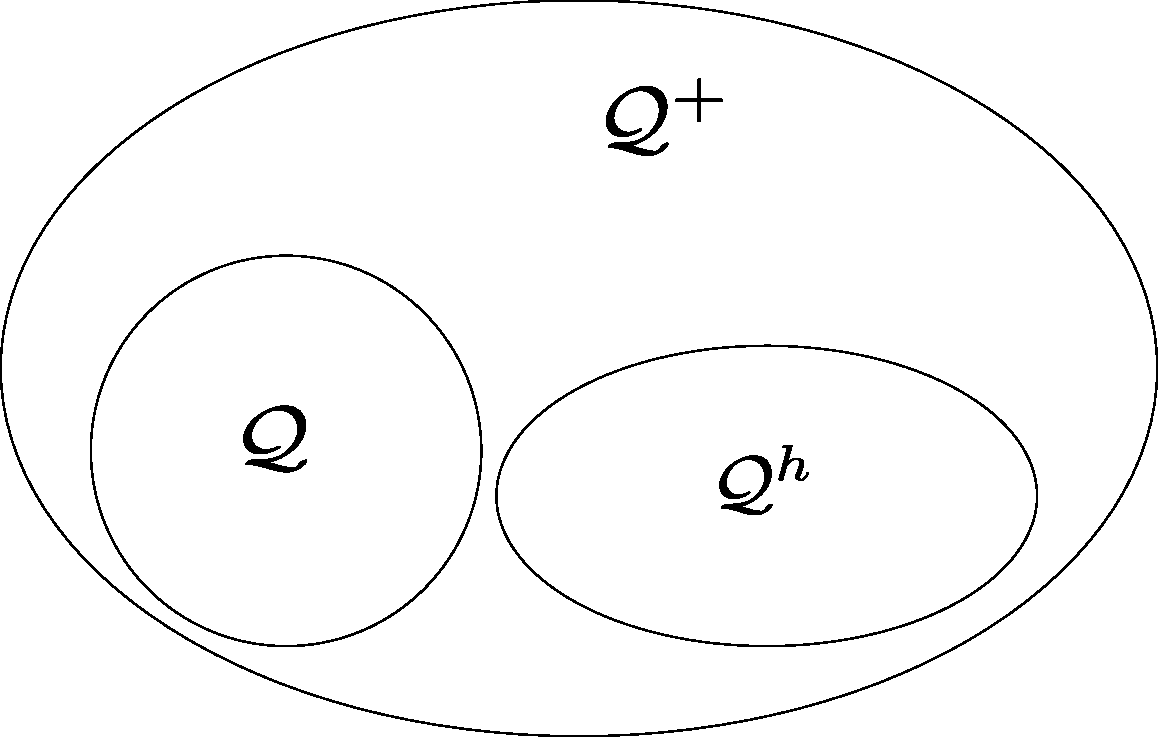
\includegraphics[width=0.90\textwidth]{slides_imgs/diagram2.pdf} 
        	\end{center}
        \end{figure}
    \end{frame}
    \begin{frame}{Variational Inference in Different Families}
        \begin{center}
            \textbf{Sparse Variational Gaussian Processes}
        \end{center}
        \[
        q^\star = \argmax_{q \in \mathcal{Q}}\  \mathbb{E}_{q(f)}[ \log p(\mathbf{y} | f)] - \text{KL}\big(q|p\big)
        \]   
        \pause
        \begin{center}
            \textbf{Decoupled Sparse Variational Gaussian Processes}
        \end{center}
        \[
        q^\star = \argmax_{q \in \mathcal{Q}^+}\ \mathbb{E}_{q(f)}[ \log p(\mathbf{y} | f)] - \text{KL}\big(q|p\big)
        \]   
        \pause
        \begin{center}
            \textbf{Fixed Mean Sparse Variational Gaussian Processes}
        \end{center}
        \[
        q^\star = \argmax_{q \in \mathcal{Q}^h}\  \mathbb{E}_{q(f)}[ \log p(\mathbf{y} | f)] - \text{KL}\big(q|p\big)
        \]   
    \end{frame}

    \begin{frame}{Variational Optimization}
        Optimizing the ELBO in the Hilbert space:
        \[
        q^\star = \argmax_{q \in \mathcal{Q}^+}\ \mathbb{E}_{q(f)} \left[ \log p(\mathbf{y}|f)\right] - \text{KL}\left(q|p\right)\,.
        \]
        where
        \[
            \text{KL}\left(q | p\right) = \frac{1}{2} \bm{a}^T \bm{K}_{\alpha} \bm{a} + \frac{1}{2} \log |\bm{I} - \bm{K}_{\beta} (\bm{A} + \bm{K}_{\beta})^{-1}| + \frac{1}{2} \text{tr}\left( \bm{K}_\beta\bm{A}^{-1} \right)
        \]
        and \(\mathbb{E}_{q(f)}\left[ \log p(\mathbf{y}|f)\right] \) can be computed in regression and estimated in classification.
    \end{frame}

    \begin{frame}{Variational Optimization}
        Optimizing the ELBO in the Hilbert space:
        \[
        q^\star = \argmax_{\color{red}q \in \mathcal{Q}^h}\ \mathbb{E}_{q(f)} \left[ \log p(\mathbf{y}|f)\right] - \text{KL}\left(q| p\right)\,.
        \]
        where
        \[
            \begin{aligned}
                \text{KL}\left(q | p\right) = \frac{1}{2} {\color{red}\bm{a}^T \bm{K}_{\alpha} \bm{a}} + \frac{1}{2} \log |\bm{I} - \bm{K}_{\beta} (\bm{A} + \bm{K}_{\beta})^{-1}| + \frac{1}{2} \text{tr}\left( \bm{K}_\beta\bm{A}^{-1} \right)
            \end{aligned}
        \]
        and \(\mathbb{E}_{q(f)}\left[ \log p(\mathbf{y}|f)\right] \) can be computed in regression and estimated in classification.
    \end{frame}

    \begin{frame}
    \begin{HighlightBoxFit}
        \(q^\star = \argmax_{q \in \mathcal{Q}^h}\ \mathbb{E}_{q(f)} \left[ \log p(\mathbf{y}|f)\right] - \text{KL}\left(q|p\right)\)
    \end{HighlightBoxFit}
    \pause
    \begin{center}
    The kernel \(\kappa_\theta(\cdot, \cdot)\) may have \textbf{hyper-parameters }\(\theta\) that affect \(q\).
    \end{center}
    \pause
    \begin{center}
        In regression: \(\kappa_{\theta}(\cdot, \cdot) \to 0\) is a \textbf{local optima} in \(\mathcal{Q}^h\).
    \end{center}
    \pause
    \begin{center}
        \textbf{Solution: \(\alpha\)-divergences}.
    \end{center}
    \end{frame}
    \begin{frame}
    \begin{HighlightBoxFit}
        \(q^\star = \argmax_{q \in \mathcal{Q}^h}\ \mathbb{E}_{q(f)} \left[ \log p(\mathbf{y}|f)\right] - \text{KL}\left(q|p\right)\)
    \end{HighlightBoxFit}
    \pause
    \vspace{-0.5cm}
    \begin{center}
          \(\Big\Downarrow\)  
    \end{center}
    \vspace{-0.5cm}
    \begin{HighlightBoxFit}
        \(q^\star = \argmax_{q \in \mathcal{Q}^h}\ \tfrac{1}{\alpha}\log \ \mathbb{E}_{q(f)} \left[  p(\mathbf{y}|f)^{\alpha}\right] - \text{KL}\left(q|p\right)\)
    \end{HighlightBoxFit}
    \pause 
    \vspace{-0.5cm}
    \begin{center}
          \(\Big\Downarrow\)  
    \end{center}
    \vspace{-0.5cm}
    \begin{HighlightBoxFit}
        \(q^\star = \argmax_{q \in \mathcal{Q}^h} \ \text{Train LL} - \text{KL}\left(q| p\right)\)
    \end{HighlightBoxFit}
    \end{frame}
    
    \begin{frame}{Intuitive Recap}
        \begin{enumerate}[<+->]\color{shadecolor}
            \item \color<.>{black}Learn a \textbf{optimal deterministic} model \(h\).
            \item \color<.>{black}Define a \textbf{Sparse Variational GP}.
            \item \color<.>{black}\textbf{Decouple the inducing locations} from the mean and covariance.
            \item \color<.>{black}Consider the \textbf{subspace with fixed mean} \(h\).
            \item \color<.>{black}Train the (non-fixed) parameters using \textbf{function-space VI} and mini-batch optimization.
            \item \color<.>{black}The resulting method \textbf{provides uncertainty estimation} for the deterministic model.
        \end{enumerate}
    \end{frame}

    % \begin{frame}{Preliminary results}
    %     \begin{figure}
    %     	\begin{center}
    %     	\begin{tabular}{ccc}
    %         {\scriptsize LLA }& {\scriptsize VaLLA }& {\scriptsize ELLA} \\
    %     	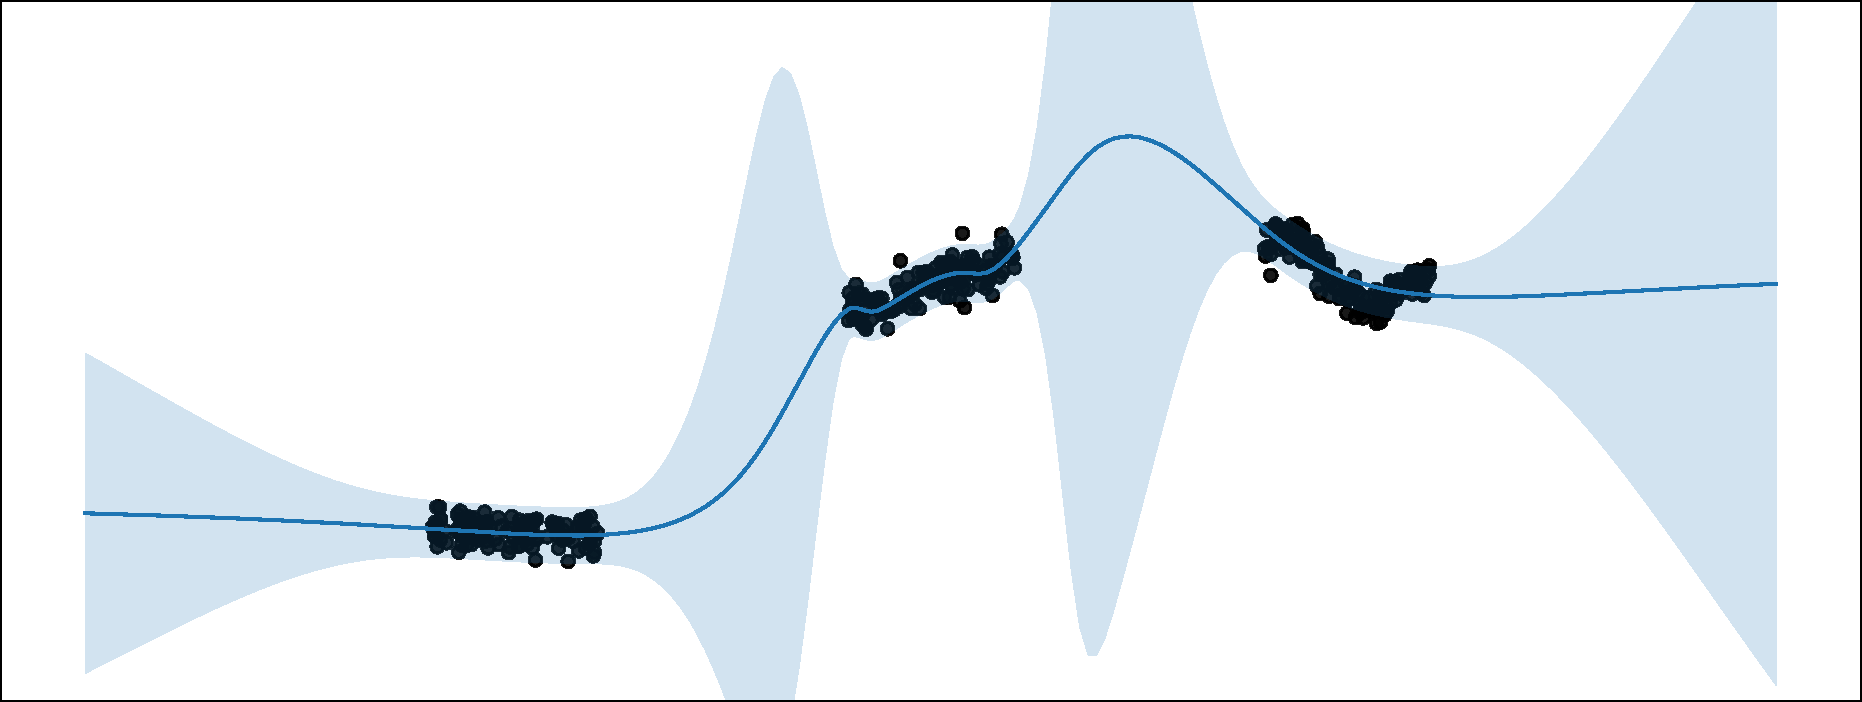
\includegraphics[width=0.30\textwidth]{imgs/LLA} & 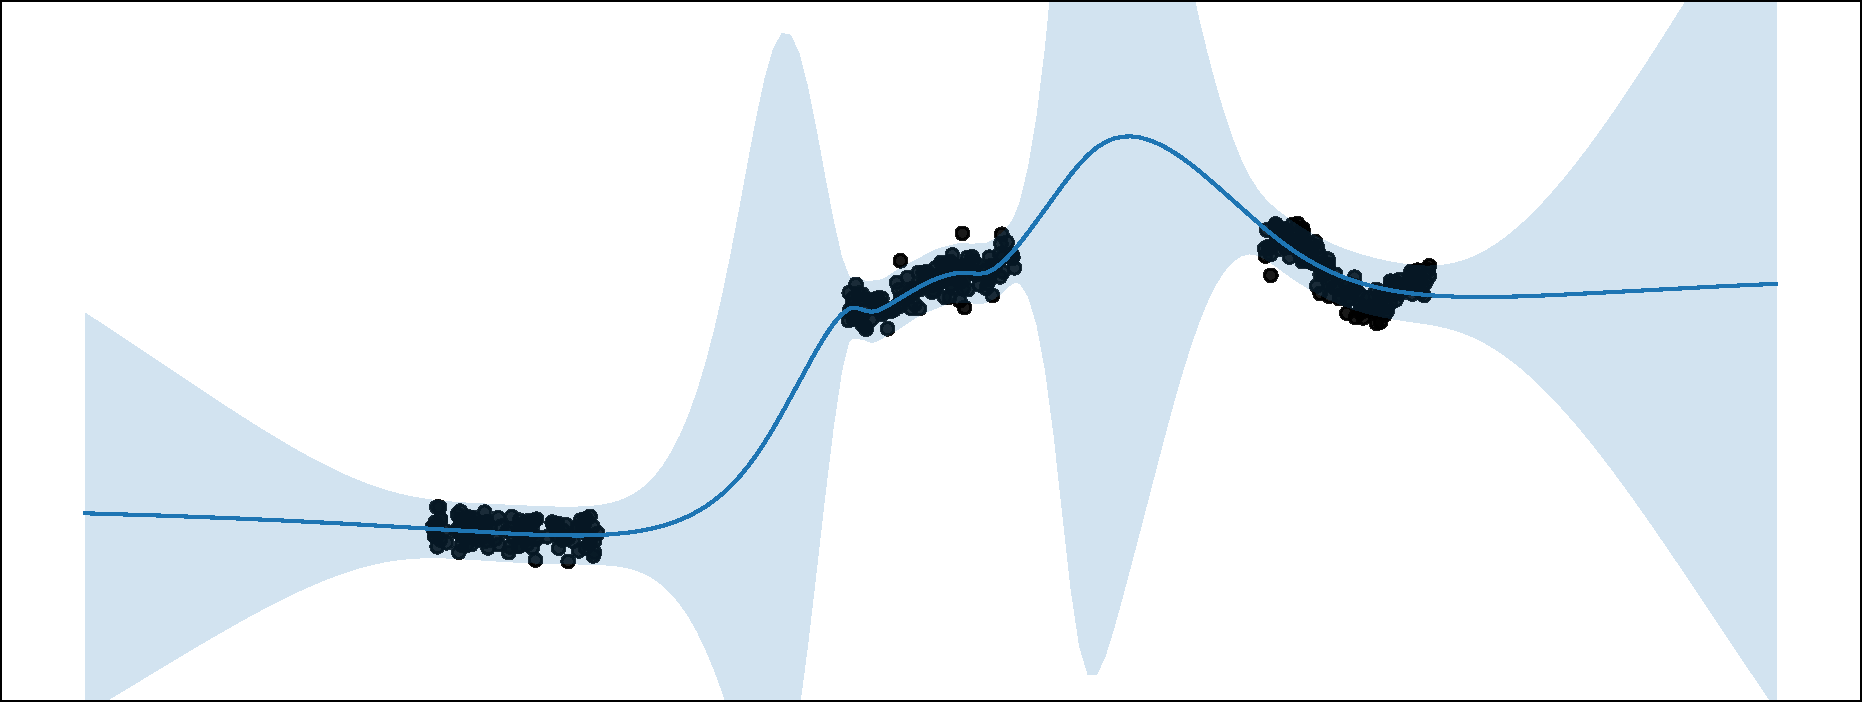
\includegraphics[width=0.30\textwidth]{imgs/VaLLA} & 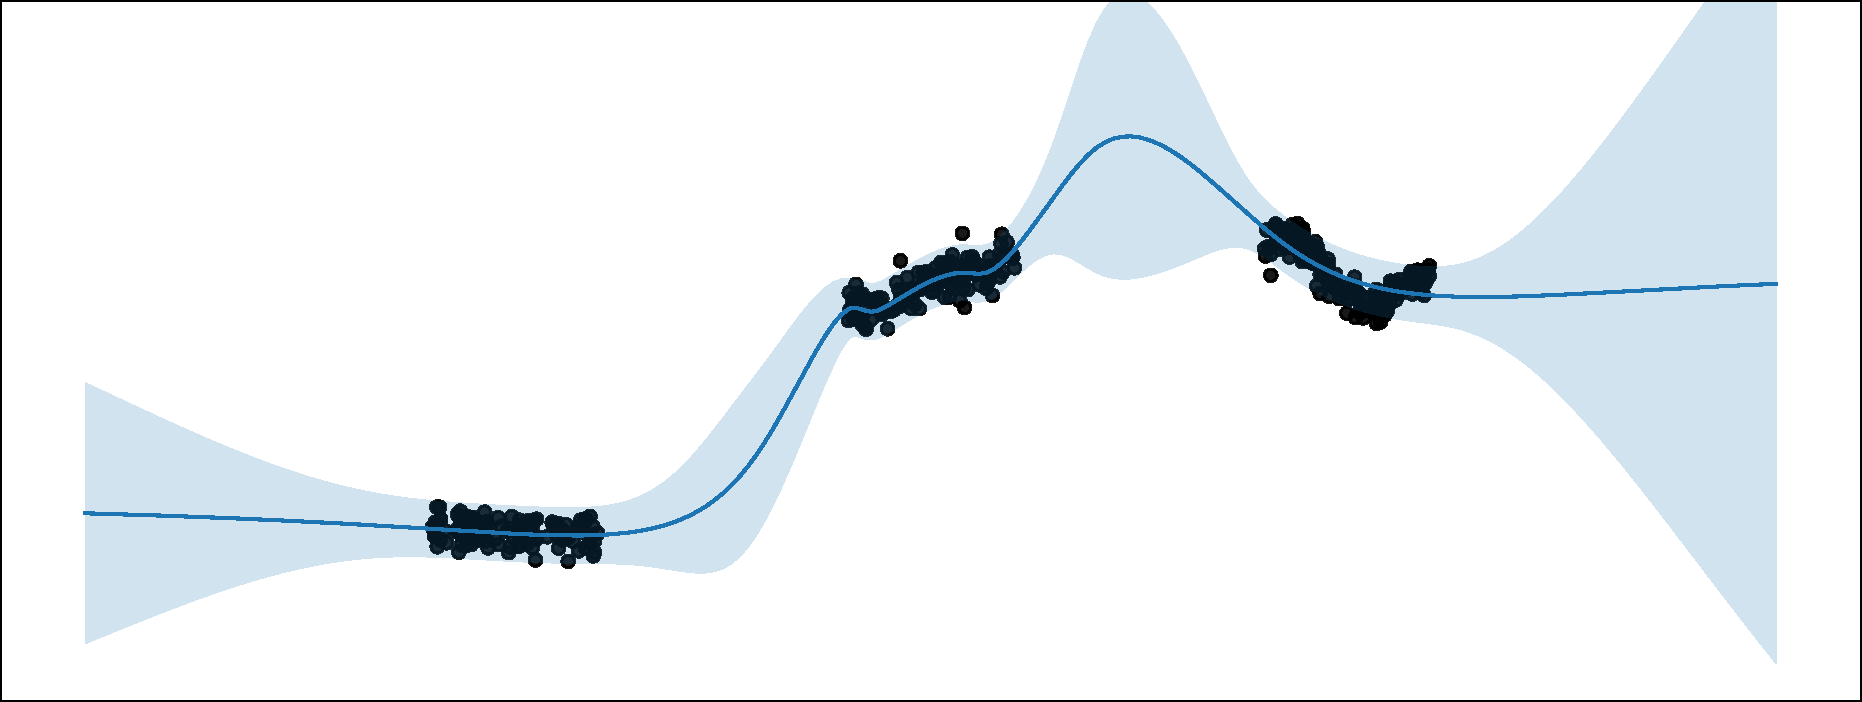
\includegraphics[width=0.30\textwidth]{imgs/ELLA.pdf} \\
    %         {\scriptsize Last-Layer LLA} & {\scriptsize Diagonal LLA} & {\scriptsize Kronecker LLA}\\
    %     	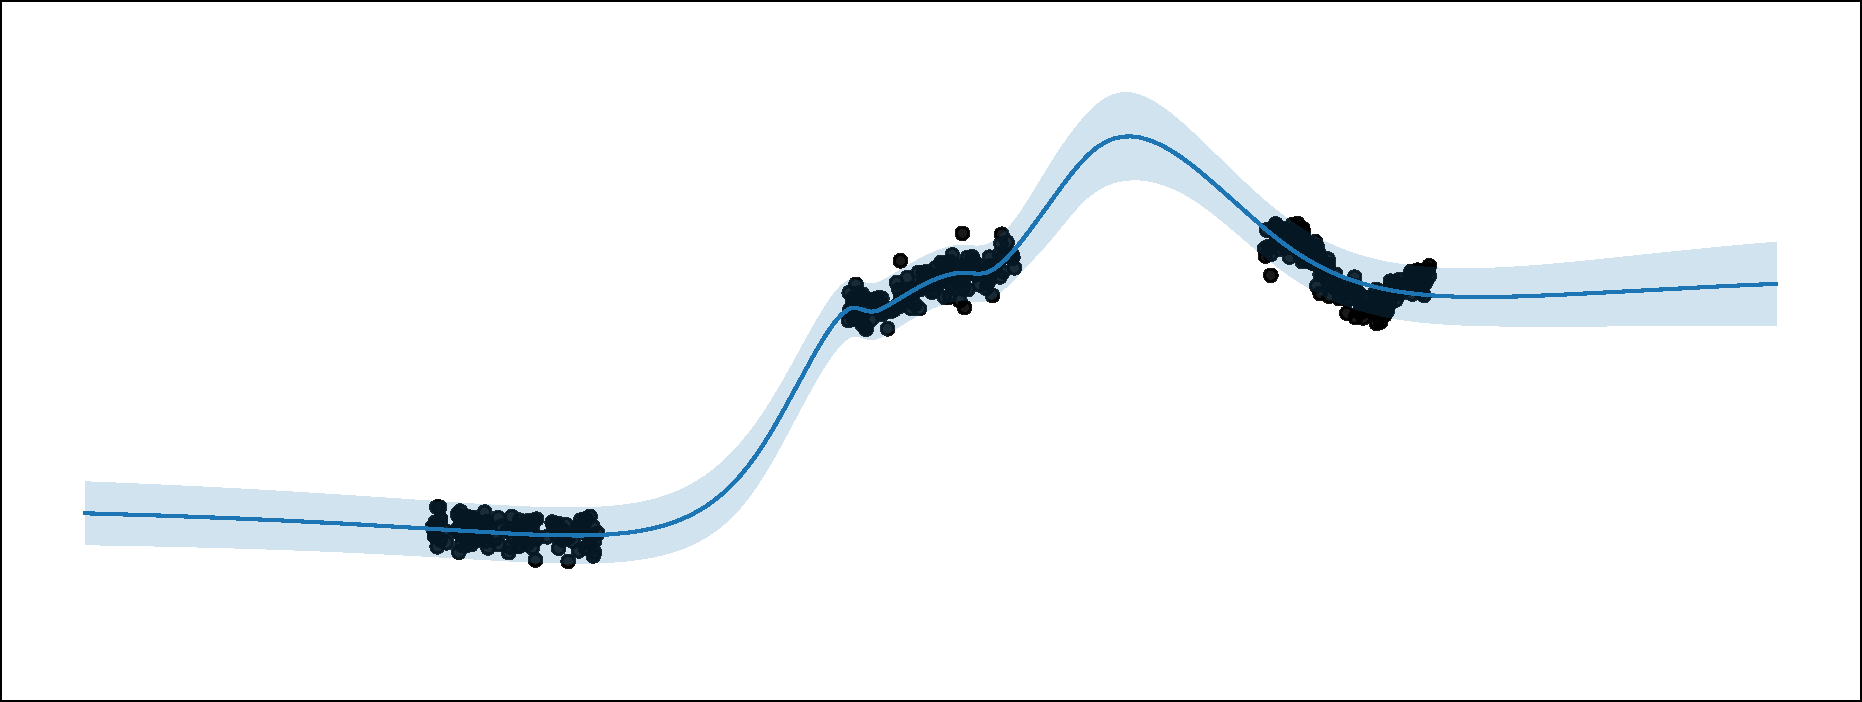
\includegraphics[width=0.30\textwidth]{imgs/LL-LLA.pdf} & 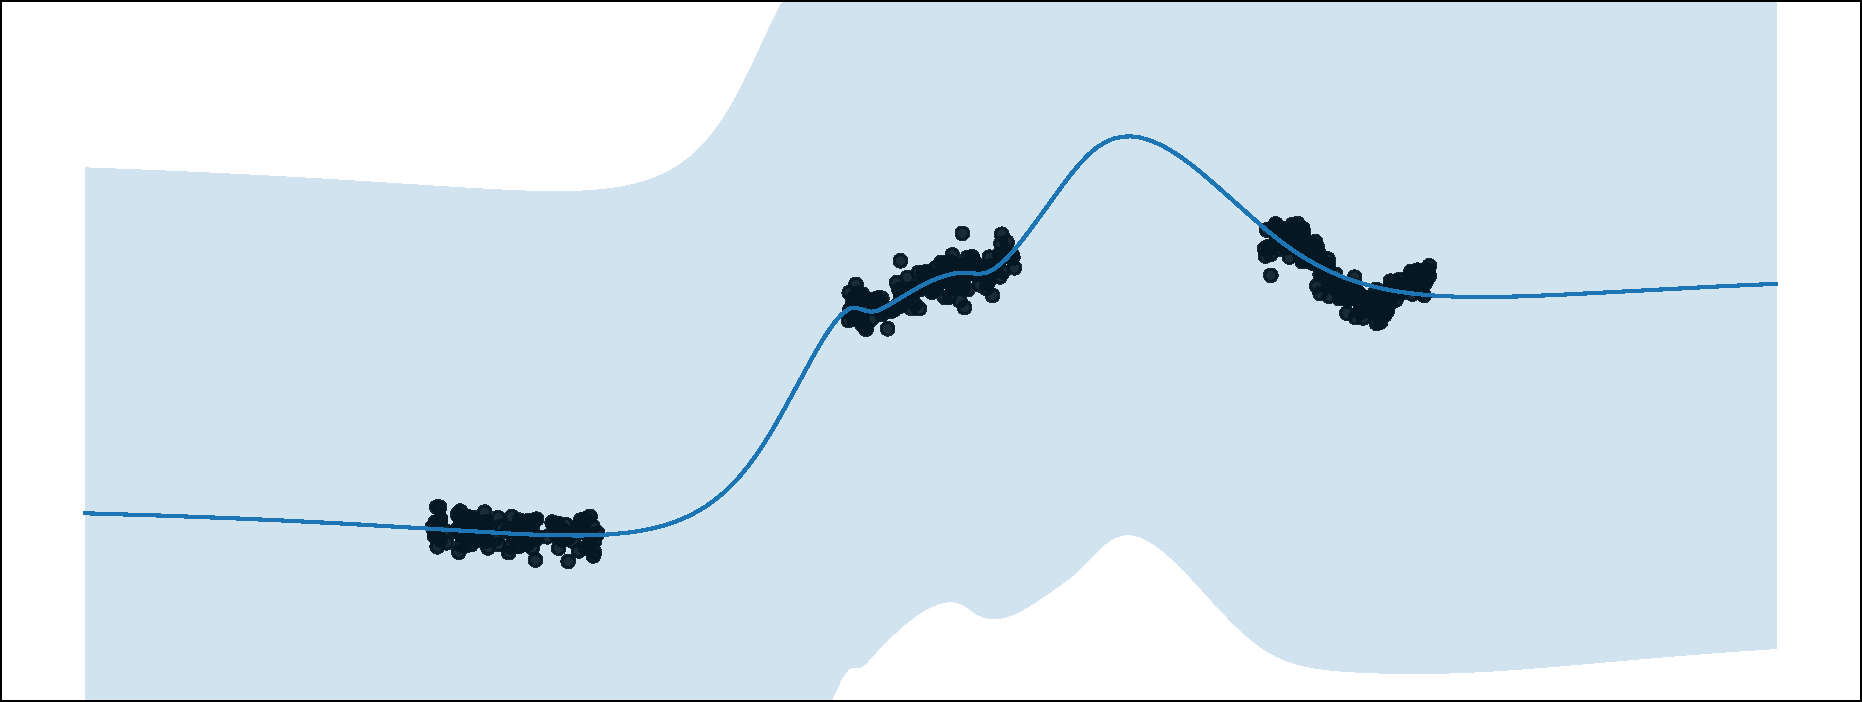
\includegraphics[width=0.30\textwidth]{imgs/Diag-LLA.pdf} & 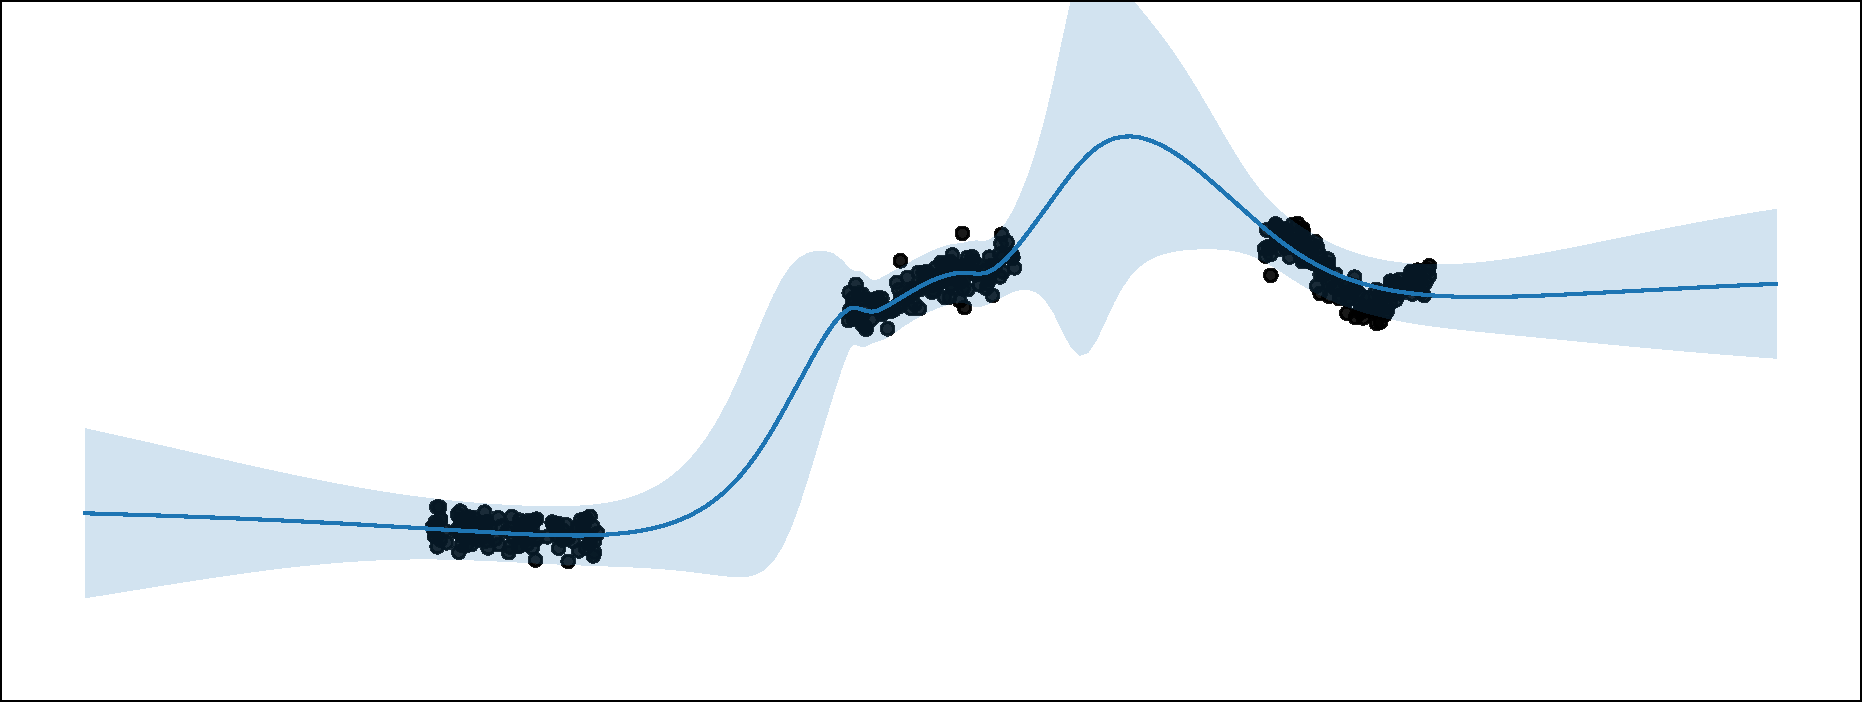
\includegraphics[width=0.30\textwidth]{imgs/LLA-KFAC.pdf} \\
    %     	\end{tabular}
    %     	\end{center}
    %         \caption{Predictive distribution (two times the standard deviation) on a toy 1D regression dataset with a 2 hidden layer MLP with \(50\) units.}
    %         \label{fig:intro}
    %     \end{figure}
    % \end{frame}
    
    \begin{frame}{Results in Regression Problems}
    \centering
    \resizebox{0.7\textwidth}{!}{\begin{tabular}{lcccccc}
        \toprule
            & \multicolumn{2}{c}{Airline} & \multicolumn{2}{c}{Year} & \multicolumn{2}{c}{Taxi} \\[0.5mm]
            \cmidrule(lr){2-3} \cmidrule(lr){4-5} \cmidrule(lr){6-7}
        Model & NLL & CRPS & NLL & CRPS & NLL & CRPS\\
        \midrule
        Deterministic       & $5.087$ & $18.436$ & $3.674$ & $5.056$& $3.763$ & $3.753$ \\
        LLA Diag  & $5.096$ & $\color{teal}\mathbf{18.317}$ & $3.650$ & $4.957$ & $3.714$ & $3.979$\\
        LLA KFAC  & $5.097$ & $\color{teal}\mathbf{18.317}$ & $3.650$ & $4.955$ & $3.705$ & $3.977$\\
        LLA$^*$   & $5.097$ & $18.319$ & $3.650$ & $\color{teal}\mathbf{4.954}$ & $3.718$ & $\color{teal}\mathbf{3.975}$ \\
        LLA$^*$ KFAC & $5.097$ & $\color{teal}\mathbf{18.317}$ & $3.650$ & $\color{teal}\mathbf{4.954}$ &  $3.718$ & $3.976$\\
        ELLA      & $5.086$ & $18.437$ & $3.674$ & $5.056$ & $3.753$ & $3.754$ \\
        VaLLA & $\color{teal}\mathbf{4.923}$ & $18.610$ & $\color{teal}\mathbf{3.527}$ & $5.071$ & $\color{teal}\mathbf{3.287}$ & $3.968$ \\
        \midrule
        This Method & $\color{purple}\mathbf{4.903}$ & $\color{purple}\mathbf{17.552}$ & $\color{purple}\mathbf{3.485}$ & $\color{purple}\mathbf{4.721}$ & $\color{purple}\mathbf{3.208}$ & $\color{purple}\mathbf{3.493}$ \\
        \bottomrule
    \end{tabular}}
    \end{frame}

    \begin{frame}{Limitations}
    \begin{HighlightBoxFit}
        \(q^\star = \argmax_{q \in \mathcal{Q}^h} \ \text{Train LL} - \text{KL}\left(q| p\right)\)
    \end{HighlightBoxFit}
    \pause
    \begin{center}
        \textbf{Regression}\\
        Zero Uncertainty \(\implies\) Train LL \(= -\infty\).
    \end{center}
    \pause
    \begin{center}
        \textbf{Multi-class Classification}\\
        Zero Uncertainty \(\implies\) Train LL \(=\) \(h\) Train LL.
    \end{center}
    \end{frame}


    \begin{frame}{Conclusions}
        \begin{enumerate}[<+->]
            \item Sparse GPs can be \textbf{characterized} in the RKHS.
            \item Sparse GPs can be generalized to \textbf{decouple the inducing points}.
            \item There exists a \textbf{subspace} with posterior mean \(h\).
            \item Preliminary results on \textbf{regression} are promising.
            \item Limited on \textbf{multi-class classification}.
        \end{enumerate}
    \end{frame}

    \begin{frame}[standout]
        Thank you for your attention!
    \end{frame}
\end{document}